\documentclass[twocolumn,amsmath,amssymb,floatfix]{revtex4}

\usepackage{natbib}
\usepackage{graphicx}% Include figure files
\usepackage{dcolumn}% Align table columns on decimal point
\usepackage{bm}% bold math
\usepackage{amssymb}
\usepackage{amsmath}
\usepackage{amsfonts}
\usepackage{epsf}
\usepackage{color} % allows color in fonts
\usepackage{verbatim}
\usepackage{listings}
\usepackage{xcolor}
\usepackage{titlesec}
\usepackage{float}
\renewcommand{\arraystretch}{1.6} % distancia vertical tablas
\usepackage[brazilian]{babel}
\usepackage[utf8]{inputenc}
\usepackage[T1]{fontenc}

\newcommand{\PAR}[1]{\left({[#1]}\right)}


\lstdefinestyle{customc}{
  belowcaptionskip=1\baselineskip,
  breaklines=true,
  frame=none,
  xleftmargin=\parindent,
  language=C,
  showstringspaces=false,
  basicstyle=\footnotesize\ttfamily,
  keywordstyle=\bfseries\color{green!40!black},
  commentstyle=\itshape\color{purple!40!black},
  identifierstyle=\color{blue},
  stringstyle=\color{orange},
}

\lstdefinestyle{customasm}{
  belowcaptionskip=1\baselineskip,
  frame=trBL,
  xleftmargin=\parindent,
  language=[x86masm]Assembler,
  basicstyle=\footnotesize\ttfamily,
  commentstyle=\itshape\color{purple!40!black},
}

\lstset{escapechar=@,style=customc}

\titlespacing\section{0pt}{12pt plus 4pt minus 2pt}{8pt plus 2pt minus 2pt}
\titlespacing\subsection{0pt}{12pt plus 4pt minus 2pt}{8pt plus 2pt minus 2pt}
\titlespacing\subsubsection{0pt}{12pt plus 4pt minus 2pt}{0pt plus 2pt minus 2pt}

\begin{document}

%%%%%%%%%%%%%%%%%%%%%%
%%%%%%%%%%%%%%%%%%%%%%
% T I T U L O
%%%%%%%%%%%%%%%%%%%%%%
%%%%%%%%%%%%%%%%%%%%%%

\title{Traçado de Gráficos e Tabelas de Convergência para Verificação a Correta Implementação de um Método Numérico}

\author{Igor Pontes Tresolavy -- NUSP 12553646 \\\small tresolavy@usp.br e Thiago Antici de Souza Rodrigues -- NUSP 12551411 \\\small tresolavy@usp.br}
\affiliation{
Escola Politécnica -- Universidade de São Paulo\\
}

\begin{abstract}
\baselineskip 11pt
Este relatório divide-se em duas partes: primeiro, demonstra-se brevemente o traçado de gráficos através de ferramentas da linguagem de programação escolhida; depois, verifica-se a convergência soluções manufaturadas para Problemas de Cauchy 1D e 2D, assim como para um Problema de Valor Inicial bidimensional sem solução explícita conhecida.
\end{abstract}

\maketitle

% Estrutura pretendida:

% Introdução
%   Solução manufaturada
%       É utilizada para depuração de métodos implementados em código
%       Testam se a ordem de convergência do método utilizado condiz com o que diz a teoria

% Boa conduta no traçado de gráficos
%   explicar o que são as boas condutas

% Tabelas de convergência - Explicação
%   Definição do erro de discretização global
%       Def. 2.5, Teorema 2.3 cap 2.3.1
%   Demonstrar ordem de grandeza do erro para h's suficientemente pequenos
%       Conseq. => espera-se que a coluna do log convirja para um valor no mínimo igual a 1 se o método estiver implementado corretamente
%   Demonstrar aproximação para estimativa de erro quando não se sabe a solução exata

% Traçado de gráficos
%   O gráfico foi construído através da interligação de pontos de "amostra" da função ao longo de passos de subdivisão do intervalo de t utilizando-se a ferramena matplotlib
%   "Como demonstração das condutas acima, utilizou-se
%    o programa '1_questao_computacional.py' para o traçado de gráficos das funções
%    $y(t) = cos(mt), -pi <= t <= pi, m E {1, 2, 3}$ para duas quantidades de
%    subdivisões do intervalo de $t$ diferentes
%    nota-se que a precisão do gráfico diminui consideravelmente com o aumento do passo dado ao longo do intervalo

% LEMBRAR DE EXPLICAR OS PARÂMETROS DO CÓDIGO AO LONGO DO TEXTO
% Cálculos das Tabelas de Convergência
%   - Dizer que o método de euler explícito foi utilizado
%   - linguagem de programacao e biblioteca
%   - analisou-se a implementação do método através de tabelas de convergência
%   - definir a solução exata e a EDO
%   - apresentar tabela de convergência
%   - gráfico
%   Para fins de verificação dos métodos implementados, definiram-se soluções manufaturadas e tabelas de convergência para Problemas de Cauchy de uma dimensão (EDO de ordem 1) e bidimensionais (EDO de ordem 2). Finalmente, utilizou-se [referencia à fórmula matemática] para análise do comportamento do método implementado em um Problema de Cauchy sem solução explícita conhecida.
%   1D
%       A solução manufaturada escolhida
%   2D
%       Para o problema bidimensional, escolheu-se $...$, correspondente ao circuito RLC abaixo
%   Desconhecido 2D
%       O problema de Lotka-Volterra não possuí solução explícita conhecida e, por isso, foi escolhido para testar-se o método

% Referências
%   Numerical Analysis (Book)
%   Numpy documentation
%   Matplotlib documentation
%   Notas de aula do prof

% APÊNDICES
%   CÓDIGO DE IMPLEMENTAÇÃO DO EULER (2.1 e 2.2)

%%%%%%%%%%%%%%%%%%%%%%
%%%%%%%%%%%%%%%%%%%%%%
\section{Introdução}
%%%%%%%%%%%%%%%%%%%%%%
%%%%%%%%%%%%%%%%%%%%%%
Ao se implementar métodos numéricos para a obtenção de soluções aproximadas de equações diferenciais em código computacional, é comum que haja a necessidade de verificar se tal método foi implementado corretamente para determinados intervalos de valores das variáveis independentes. Uma das maneiras de realizar tal tarefa consiste na comparação do comportamento do erro de aproximação entre soluções exatas conhecidas e soluções estimadas pelo código desenvolvido, tendo em vista o comportamento esperado previsto em teoria de métodos numéricos. Tal método de verificação é denominado Método de Solução Manufaturada \cite{livroProfAlexandre}.

Ademais, como uma forma de visualização dos métodos implementados, gráficos podem ser utilizados. O traçado de gráficos para diferentes níveis de precisão da aproximação do código computacional permite a observação do comportamento convergente (ou não convergente) do método, dado que, para níveis de precisão maiores, as soluções aproximadas tendem a atenuar a redução do erro do método, caso esse tenha sido implementado corretamente no intervalo de valores da variável independente desejado. O traçado de gráficos, no entanto, é melhor aproveitado caso boas práticas de apresentação sejam seguidas \cite{tarefaProfAlexandre}.

Este relatório apresenta normas de "boa conduta" no traçado de gráficos e exemplifica-as no âmbito da verificação de códigos computacionais para a aproximação de soluções de equações diferenciais unidimensionais e bidimensionais através do método de passo único de Euler.


Este trabalho apresenta alguns resultados da aplicação de três métodos de passo único, aplicados a uma EDO particuar, para analisar o comportamento e a convergência das soluções em relação ao tamanho do passo de integração. Uma breve descrição de cada método é dada na seguinte seção, seguida por uma descrição concisa da implementação numérica utilizada para estudar estes métodos. Depois, na seção \ref{sec:exemplosnum}, os resultados numéricos obtidos são mostrados com alguns gráficos e, finalmente, finalmente são apresentados dois procedimentos de estimativa da ordem de convergência a partir dos resultados numéricos.

\section{Boa conduta no traçado de gráficos}
\label{sec:boaCondutaGraficos}

\section{Tabelas de convergência}
\label{sec:tabelasDeConvergencia}

\section{Traçado de gráficos}
\label{sec:tracadoDeGraficos}

\section{Exemplificando Tabelas de Convergência}
\label{sec:tabelasDeConvergencia}

\subsection{Método de Solução Manufaturada}
\label{subsec:solucaoManufaturada}

\subsubsection{EDO 1D}
\label{subsubsec:edo1D}

\subsubsection{Sistema 2D de EDOs}
\label{subsubsec:sistemaDeEdos2D}

\subsection{Sistema 2D de EDOs sem solução exata conhecida}
\label{subsec:sistemaEdoDesconhcido}

\section{Conceitos generais}
Nesta seção, apresentaremos brevemente os três métodos de uma etapa com os quais trabalharemos neste relatório.

Dado o seguinte problema de valor inicial (PVI) na forma normal:
\begin{eqnarray}
\frac{y(t)}{dt}=f(t, y(t)) \quad \text{com} \quad y(t_0)=y_0,
\end{eqnarray}
definido em $[t_0,T]\subset \mathbb{R}$.
Um método de passo único tem a forma geral:
\begin{equation}
\left\{\begin{array}{rl}
    y_0 &= y(x_0)  \\
    y(t_{k+1}) &= y(t_{k})+h\phi(t_k,t_{k+1},y_k,y_{k+1},h),
\end{array}\right.
\end{equation}
onde $k=0,...,n-1$; $t_{k+1}=t_k+h$ e $h=(T-t_0)/n$. Sendo $n$ o número de subintervalos de uma partição do intervalo $[t_0,T]$.

\subsection{Método de Euler}
O Método de Euler estima uma solução numérica a partir da noção b\'asica de derivada, i. e.,
podemos aproximar y'(t) por:
\begin{eqnarray}
\frac{y(t)}{dt}\approx \frac{y(t+\Delta t)-y(t)}{\Delta t}.
\end{eqnarray}
Como $\dot y(t)$ é igual a $f(t, y(t))$, por definição. Então o método de Euler é da seguinte forma:
\begin{eqnarray}
y_{k+1}= y_k + h(t_k, y_k);\quad k=0,...,n-1.
\end{eqnarray}
Para uma partição do intervalo $[t_0,T]$ em $n$ subintervalos de tamanho $n=(T-t_0)/n$. Neste caso, $\phi(t_k,y_k)=f(t_k,y_k)$.

No método de Euler, cada aproximação da solução em cada passo é feita somente usando valores no instante imediatamente anterior, pelo que este método denomina-se também, método explícito.

Em seguida apresentaremos dois métodos que envolvem não apenas o termo anterior, mas também o termo do instante atual e são chamados de métodos implícitos.

\subsection{Método de Euler Implícito}
Neste método, a função de discretização $\phi(t_{k+1},y_{k+1})=f(t_{k+1},y_{k+1})$ depende também do valor da solução aproximada no instante atual $t_{k+1}$ e tem a forma
\begin{equation}
\left\{\begin{array}{rl}
    y_0 &= y(x_0)  \\
    y_{k+1} &= y_{k}+hf(t_k,t_{k+1}),
\end{array}\right.
\end{equation}

\subsection{Método do Trapézio Implícito}
O processo iterativo do método do trapézio implícito é da forma
\begin{equation}
\left\{\begin{array}{rl}
    y_0 &= y(x_0)  \\
    y_{k+1} &= y_{k}+h\left( \frac{f(t_k,y_k)+f(t_k,t_{k+1})}{2}\right),
\end{array}\right.
\end{equation}

Os dois últimos métodos implícitos apresentados impõem a necessidade de utilizar algum outro método para aproximar $y_{k+1}$ em cada passo de integração, pois este também está presente no segundo membro da equação do método.

Portanto, neste trabalho, estes dois últimos métodos serão tratados em conjunto com o método do ponto fixo.

\subsection{Método do Ponto Fixo}
Um numero $p\in\mathbb{R}$ é um ponto fixo de uma função $g:\mathbb{R}\to\mathbb{R}$, se $g(p)=p$.
Além disso, se definirmos a relação de recorrência
\begin{equation}
    x_{i+1}=g(x_i),\quad i=0,1,2,...
\end{equation}
onde $x_0$ é uma aproximação inicial da raiz da função $f(x)=g(x)-x=0$.

A expressão anterior pode ser usada para aproximar a raiz da função $f$, sempre que exista um ponto fixo para $g$.

Neste artigo não aprofundaremos teoricamente a convergência deste método, mas apenas as provas nos exemplos numéricos que serão apresentados na próxima seção.
%%%%%%%%%%%%%%%%%%%%%%
%%%%%%%%%%%%%%%%%%%%%%
\section{Implementação dos métodos}
%%%%%%%%%%%%%%%%%%%%%%
%%%%%%%%%%%%%%%%%%%%%%
O algoritmo para os métodos foi implementado na linguagem \textit{Python} em um arquivo único.
Os gr\'aficos foram gerados usando a biblioteca \textit{matplotlib} do \textit{Python}.

%%%%%%%%%%%%%%%%%%%%%%
\subsection{Funções do programa}
%%%%%%%%%%%%%%%%%%%%%%
Abaixo segue um breve resumo do conte\'udo das principais funções do c\'odigos fonte do programa.
\\\indent \textbf{ Tarefa2.py:} Contem todas as funções que realizam os métodos numéricos no programa.
Um pedaço de sua interface é apresentado a seguir:

\textbf{Função do método de Euler}
\begin{lstlisting}[language=Python]
#   METODO DE EULER
def Euler(vt,vy0,dt):                  # Methodo de Euler
    # vt: vetor tempo, vy0: vetor inicial, dt: tamanho passo
    ys=vy0.copy()                      # inicailizacao vetor solucao
    for i in range(len(vt)-1):
        ys.append(ys[i]+dt*f(vt[i],ys[i]))
    return np.array(ys)
\end{lstlisting}

\textbf{Função do Método de Euler Implícito}
\begin{lstlisting}[language=Python]
#   METODO EULER IMPLICITO
def EulerImp(vt,vy0,dt):               # npf: iteracoes ponto fixo
    # vt: vetor tempo, vy0: vetor inicial, dt: tamanho passo
    npf=6
    ys=vy0.copy()
    for i in range(len(vt)-1):
        y0_pf=ys[-1]+dt*f(vt[i],ys[-1])   # chute inicial(usando Euler) para usar ponto fixo
        yPonFix=y0_pf.copy()              # Inicio Methodo ponto fixo
        for j in range(npf):
            yPonFix=ys[-1]+dt*f(vt[i]+dt,yPonFix)
        ys.append(yPonFix)                # Fim Metodo ponto Fixo
    return np.array(ys)
\end{lstlisting}

\textbf{Função do Método do Trapézio Implícito}
\begin{lstlisting}[language=Python]
#   METODO TRAPEZIO IMPLICITO
def TraImp(vt,vy0,dt):
    npf=6
    ys=vy0.copy()
    for i in range(len(vt)-1):
        y0_pf=ys[-1]+dt*f(vt[i],ys[-1]) # chute inicial(usando Euler) para usar ponto fixo
        yPonFix=y0_pf.copy()            # Inicio Methodo ponto fixo
        for j in range(npf):
            yPonFix=ys[-1]+dt*(f(vt[i],ys[-1])+f(vt[i]+dt,yPonFix))/2
        ys.append(yPonFix)              # Fim Metodo ponto Fixo
    return np.array(ys)
\end{lstlisting}
%%%%%%%%%%%%%%%%%%%%%%

%%%%%%%%%%%%%%%%%%%%%%
\subsection{Parâmetros e execução do programa}
%%%%%%%%%%%%%%%%%%%%%%
O programa inicia, pedindo para escolher o método a ser utilizado e o tempo final $T$, onde o intervalo de solução é $[t_0,T]$.
Em seguida, a saída do programa são dois diagramas que mostram as soluções reais e numéricas para alguns valores de passos de integração e uma tabela com os valores de erro e uma aproximação da ordem de convergência.

Nos métodos Euler e trapezoidal implícito, o número de iterações feitas utilizando o método do ponto fixo foi $6$ e como chute inicial usou-se o método de Euler. Vale lembrar, entretanto, que os resultados obtidos usando o método de ponto fixo convergiram somente para valores de $h$ muito pequenos e mais rapidamente para o método do trapézio.

Para validar o c\'odigo numérico para aplicações reais, foram usados tamanhos de passo $h=(T-t_0)/2^m$, com $m=5,6,7,...,15$.
Conforme este $m$ aumentava, as aproximações melhoravam, mas com um custo no tempo de execução. Portanto, optou-se por utilizar apenas o conjunto de valores mencionados acima.
Além disso, foi considerada uma EDO com solução analítica conhecida que se apresentara na seguinte seção.

%%%%%%%%%%%%%%%%%%%%%%
%%%%%%%%%%%%%%%%%%%%%%
\section{Exemplos Numéricos}\label{sec:exemplosnum}
Em todos os exemplos a seguir, é considerado o seguinte problema de Cauchy:
\begin{equation}\label{eq:EDO}
\left\{\begin{array}{ll}
    x' = y, & x(\sqrt{\pi})=0\\
    y' = y/t-4t^2x, & y(\sqrt{\pi})=-2\sqrt{\pi},
\end{array}\right.
\end{equation}
com $t\in[\sqrt{\pi}, T]$. Com solução exata dada por
\begin{equation}
    (x(t),y(t))=(sin(t^2),2tcos(t^2)),\quad t\in[\sqrt{\pi}, T].
\end{equation}

\subsection{Problema de Cauchy com solução exata conhecida}\label{sec:PVIConSol}
%%%%%%%%%%%%%%%%%%%%%%
%%%%%%%%%%%%%%%%%%%%%%
Neste caso, os instantes $T=3$ e $T=5$ foram considerados para calcular a ordem de convergência em cada método. Além disso, a estratégia de verificação por solução manufaturada é usada (ver \cite{livroProfAlexandre}).

Apresentaremos tabelas com os erros globais variando o tamnaho so passo de integração $h=(T-\sqrt{\pi})/2^m$, $m=5,6,7,...,15$.

Para o cálculo do erro global, em todos os exemplos numéricos desta seção ($A$), foi utilizada a norma do máximo, ou seja, dado $e(t,h)=(e_x(t,h),e_y(t,h))$, então para $h$ e $t$ fixos,
\begin{equation}
    \|e(t,h)\|=\max\{|e_x(t,h)|,|e_y(t,h)|\}.
\end{equation}

\subsubsection{Resultados do Método de Euler}
As Figuras \ref{fig:m1t3} e \ref{fig:m1t5} mostram o comportamento das soluções numéricas para as variáveis $x$ e $y$, respectivamente, para uma partição de $n=32,512,2048$ do intervalo solução $[\sqrt{\pi},5]$. Como se pode ver, à medida que $t$ aumenta, as soluções numéricas começam a ficar piores.

Aplicando o Método Euler e considerando um instante fixo $T=3$, ver Tabela \ref{tab:m1t3}, notamos que à medida que $n$ cresce, ou seja, o valor de $h$ diminui, observamos uma diminuição do erro, também o quociente $q$ entre erros considerando um passo de tamanho $2h$ e $h$, vai para $2$, o que nos faz perceber um crescimento linear do tamanho do passo em relação ao erro.
Também pela teoria da expansão assimptótica do erro, ver \cite{livroProfAlexandre}, temos que a ordem de convergência $p$ deste método pode ser aproximada como
\begin{equation}
    p\approx \log_2 \frac{\|e(t,2h)\|}{\|e(t,h)\|}.
\end{equation}
As Tabelas \ref{tab:m1t3} e \ref{tab:m1t5} mostram uma estimativa do valor de $p\approx 1$ y como os erros variam em função do tamanho de passo de integração $h$ para os instantes $T=3$ e $T=5$ respetivamente.

\begin{figure}[H]
\centering
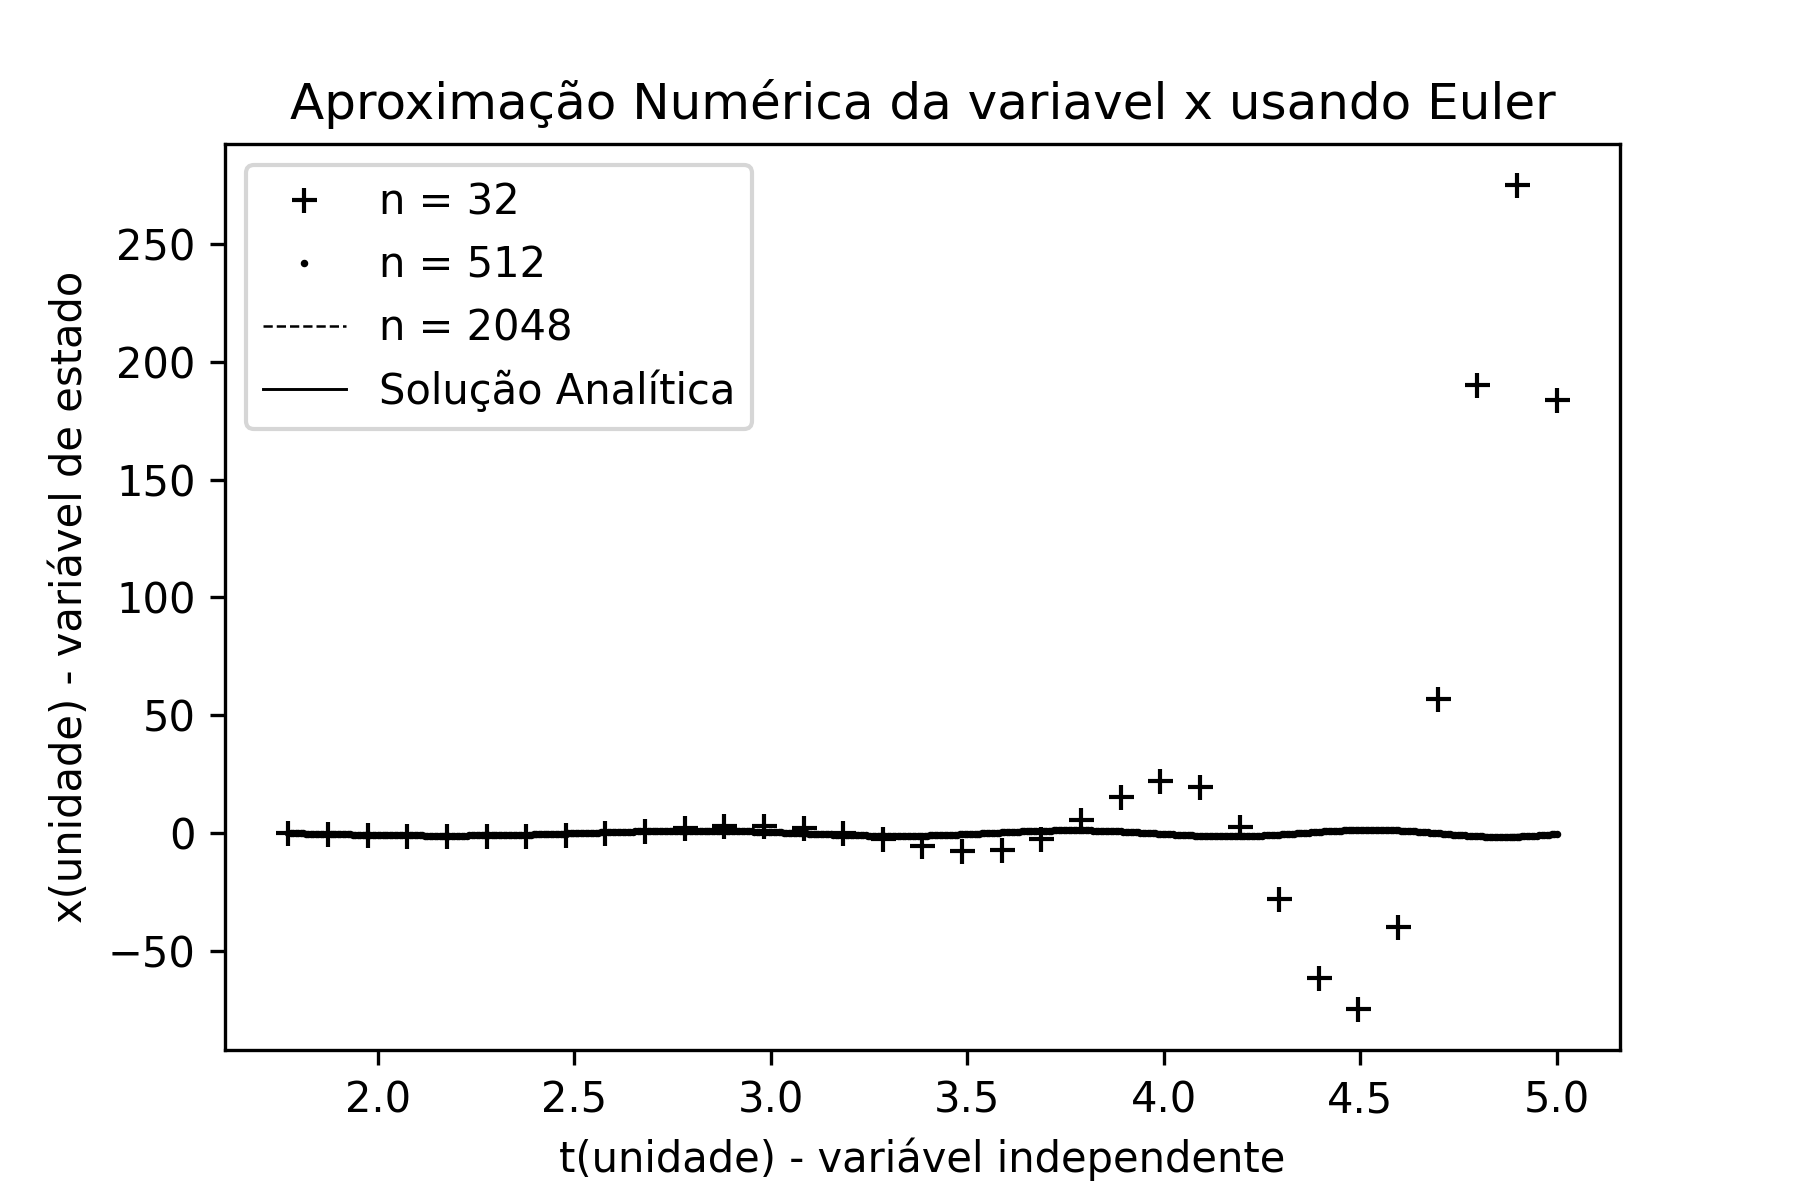
\includegraphics[scale=0.55]{images/metodo_1x_T5.0.png}
\caption{Aproximações numéricas da variável $x$ no intervalo $[\sqrt{\pi},5]$ para o Método de Euler.}
\label{fig:m1t3}
\end{figure}

\begin{figure}[H]
\centering
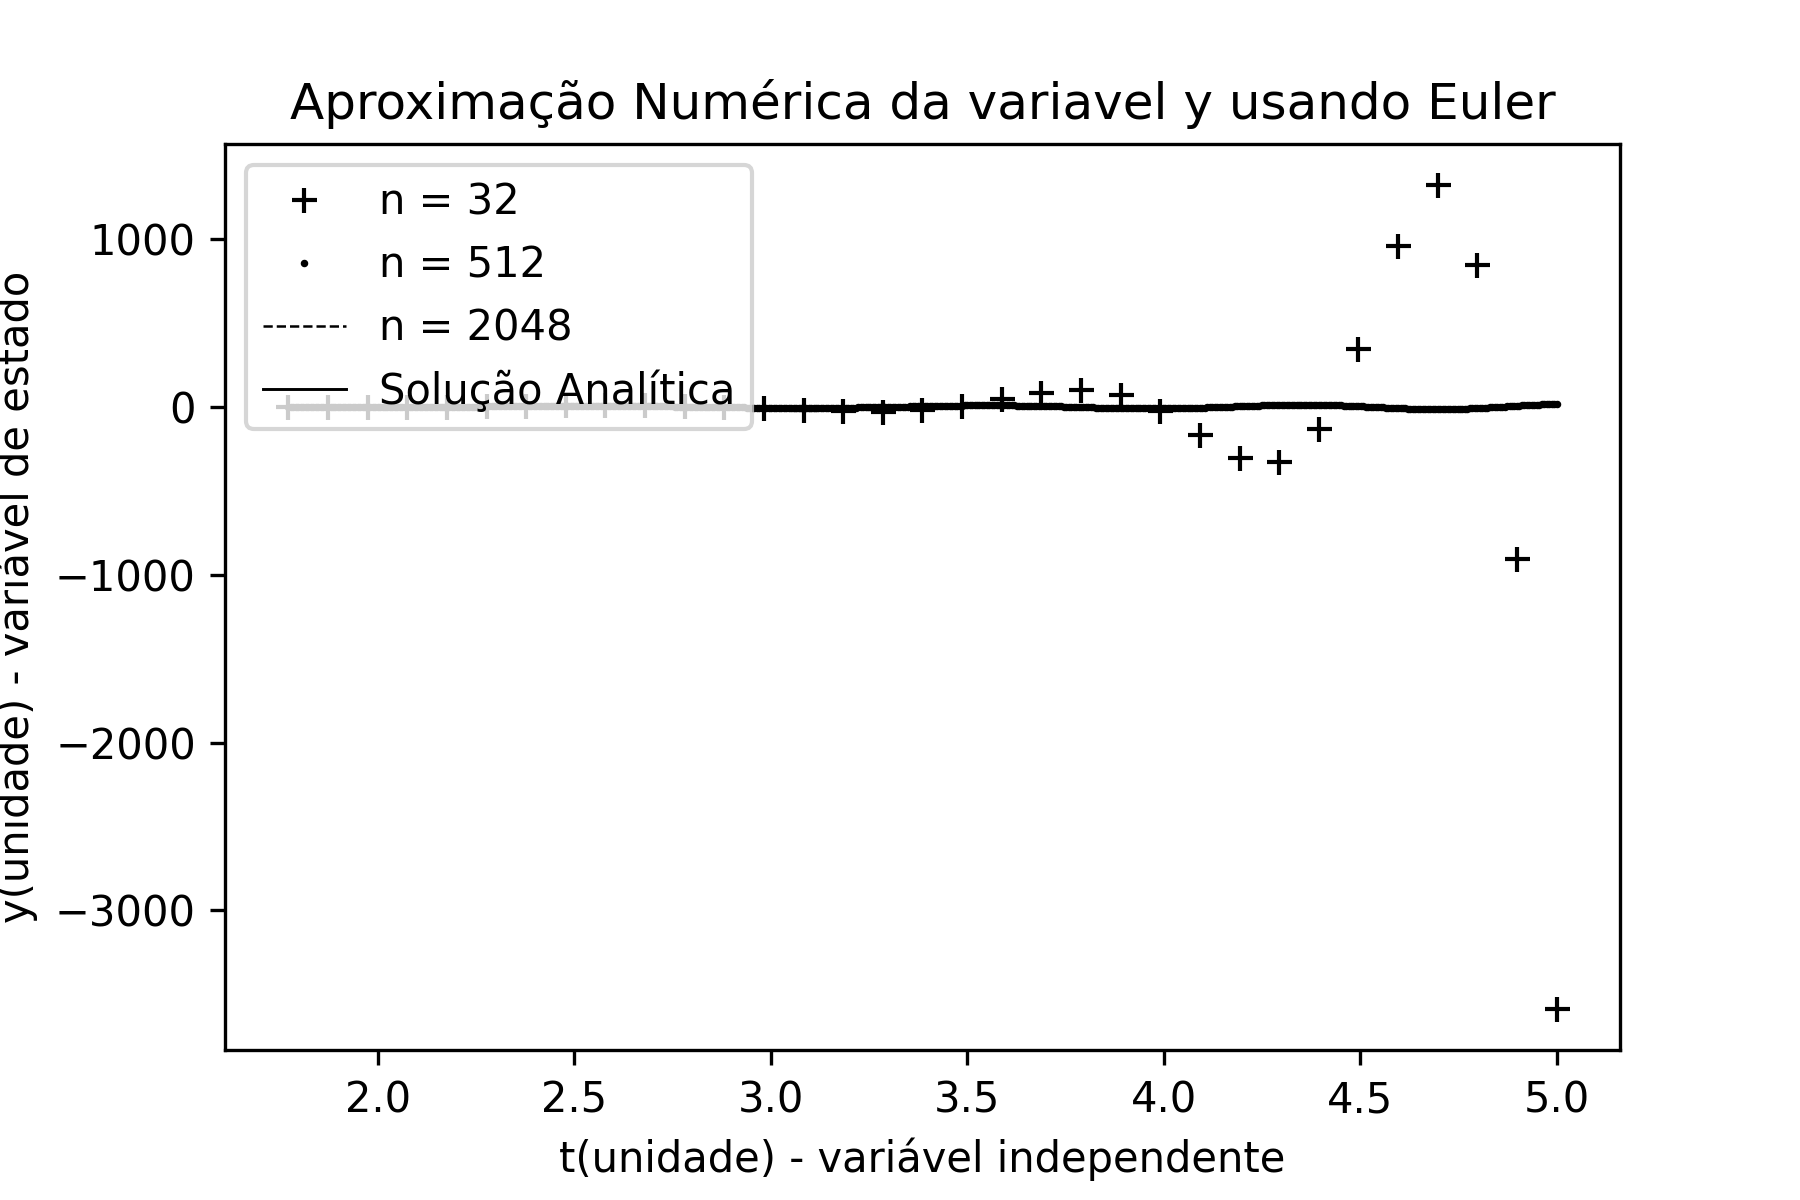
\includegraphics[scale=0.55]{images/metodo_1y_T5.0.png}
\caption{Aproximações numéricas da variável $y$ no intervalo $[\sqrt{\pi},5]$ para o Método de Euler.}
\label{fig:m1t5}
\end{figure}

%   TABELA EULER T=3
\begin{table}[H]
 \centering
 \begin{tabular}{ c|c|c|c }
  \hline
  \hline
  $n$  & $\|e(t,h)\|$  & $q=\frac{\|e(t,2h)\|}{\|e(t,h)\|}$ & $\log_2(q)$ \\
  \hline
  \hline
 $32$ & $2.990645374$ & & \\
  \hline
 $64$ &	$1.471219698$ &	$2.032765995$	& $1.023444147$  \\
   \hline
 $128$&	$0.71758463$ &	$2.050238587$	& $1.035791807$\\
\hline
$256$&	$0.353200997$ & $2.031660826$&$	1.022659572$\\
\hline
$512$&	$0.175091685$ & $2.017234558	$&$1.012378846$\\
\hline
$1024$&$0.087156235$ & $2.008940442	$&$1.006434794$\\
\hline
$2048$&	$0.043479254$&	$2.004547604$ & $1.003276679$\\
\hline
$4096$&	$0.021714734$ & $2.002292727	$ & $1.001652906$\\
\hline
$8192$&	$0.010851122$ &	$2.001151042	$ & $1.000830063$\\
\hline
$16384$&	$0.005423997$ & $2.000576684	$ & $1.00041593$\\
\hline
$32768$&	$0.002711607$ & $2.000288632	$ & $1.000208189$ \\
  \hline
  \hline
 \end{tabular}
   \caption{Estimação da ordem de convergência do Método de Euler no instante $T=3$, para o PVI com solução conhecida.} \label{tab:m1t3}
\end{table}

%   TABELA EULER T=5
\begin{table}[H]
 \centering
 \begin{tabular}{ c|c|c|c }
  \hline
  \hline
  $n$  & $\|e(t,h)\|$  & $q=\frac{\|e(t,2h)\|}{\|e(t,h)\|}$ & $\log_2(q)$ \\
  \hline
  \hline
$32$&$3595.491729$&	$$ &	$$ \\
\hline
$64$&$66.29462666$&$	54.23504$&$	5.761153339$\\
\hline
$128$&$49.89709896$&$	1.328626875$&$	0.409936002$\\
\hline
$256$&$16.04842414$&$	3.109158788$&$	1.636524298$\\
\hline
$512$&$6.281958983$&$	2.554684643$&$	1.353145212$\\
\hline
$1024$&$2.779297721$&$	2.260268461$&$	1.176494138$\\
\hline
$2048$&$1.307932377$&$	2.124955212$&$	1.087432434$\\
\hline
$4096$&$0.634572891$&$	2.061122364$&$	1.043430157$\\
\hline
$8192$&$0.312563997$&$	2.030217483$&$	1.021634282$\\
\hline
$16384$&$0.155116888$&$	2.015022354$&$	1.010795844$\\
\hline
$32768$&$0.077269089$&$	2.007489531$&$	1.005392464$\\
  \hline
  \hline
 \end{tabular}
   \caption{Estimação da ordem de convergência do Método de Euler no instante $T=5$, para o PVI com solução conhecida.} \label{tab:m1t5}
\end{table}


\subsubsection{Resultados do Método de Euler Implícito}

O método de Euler implícito parece apresentar melhores resultados em comparação com o método Euler, isto pode ser visto nas Figuras \ref{fig:m2t3} e \ref{fig:m2t5}.
O que pode ser visto mais claramente nas Tabelas \ref{tab:m2t3} e \ref{tab:m2t5}, onde os erros são menores em comparação com o método do Euler para os mesmos instantes fixos $T=3$ e $T=5$.
Como a análise feita acima, estas tabelas nos permitem fazer uma estimativa da ordem de convergência do método de Euler e implícito, sendo também aproximadamente $p=1$.

\begin{figure}[H]
\centering
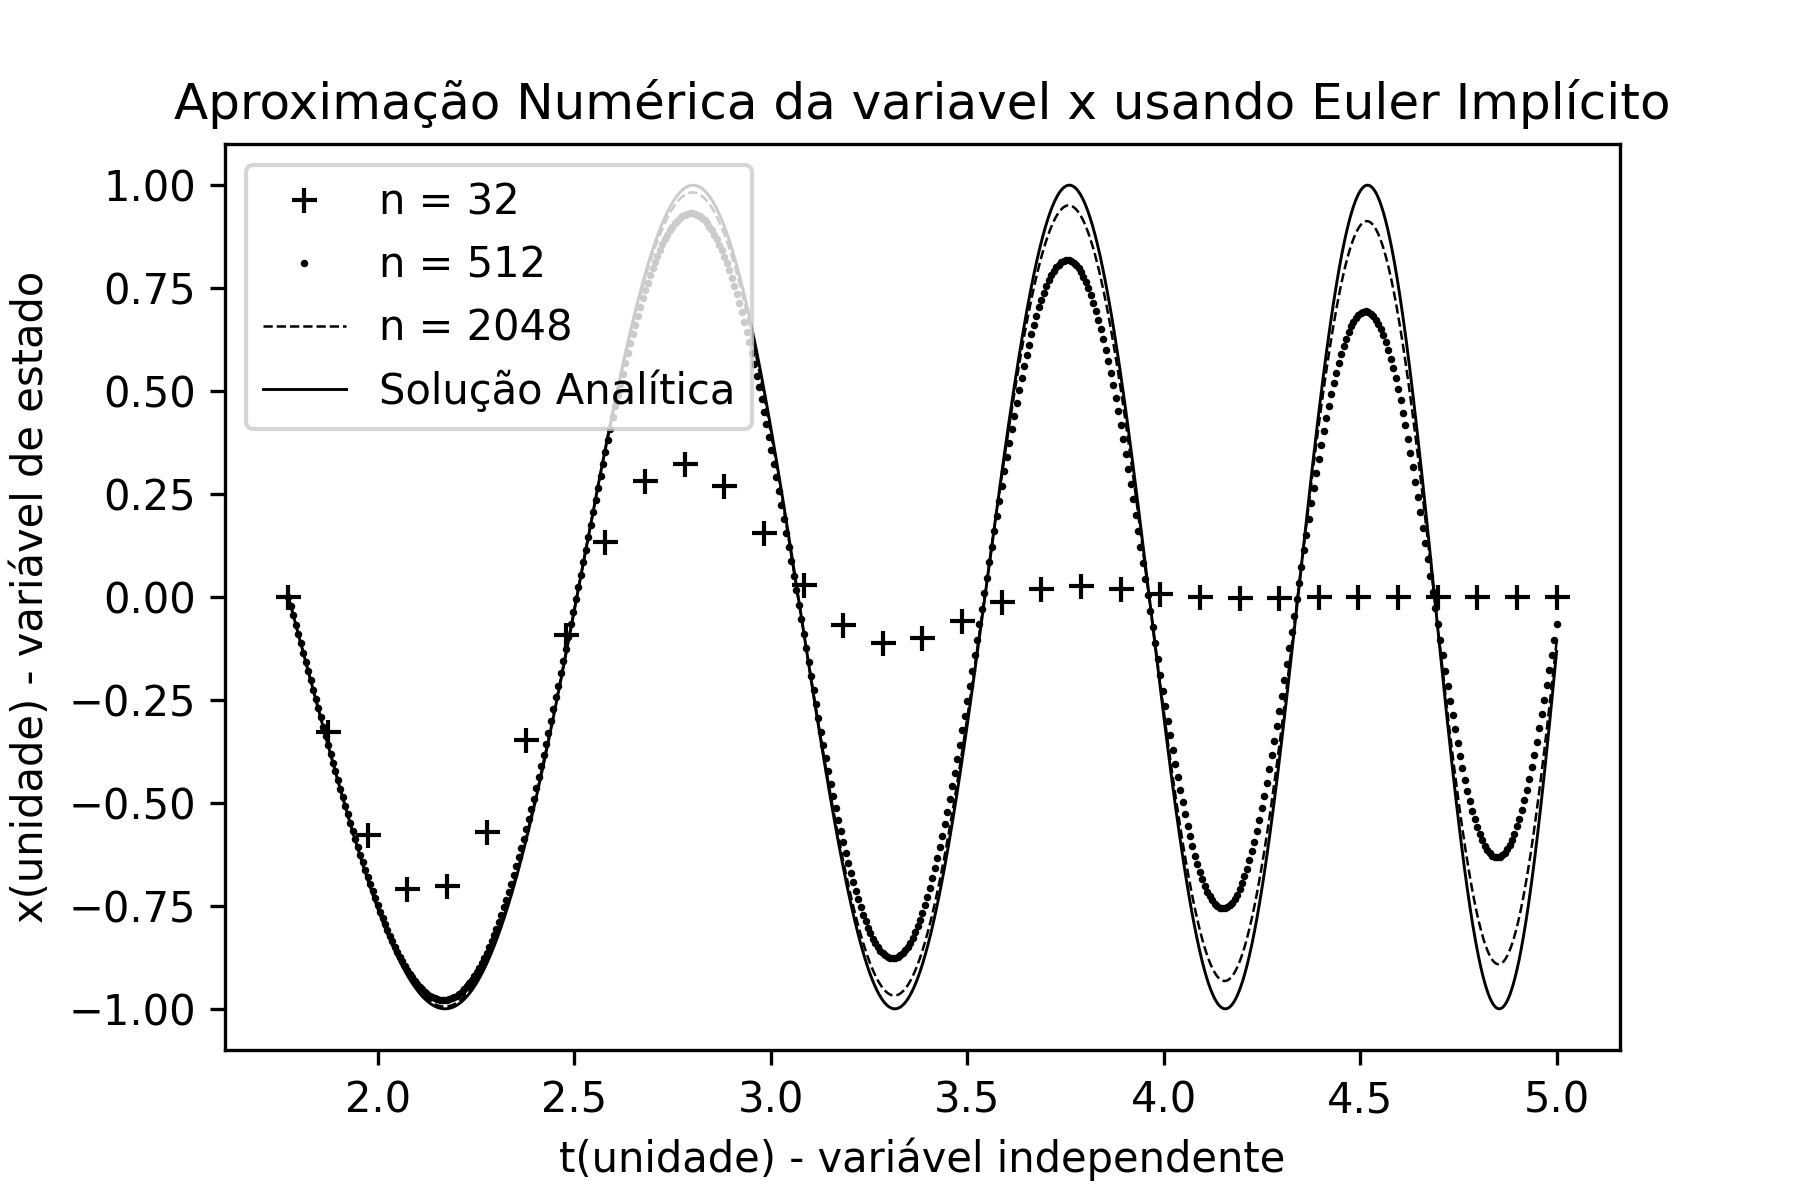
\includegraphics[scale=0.55]{images/metodo_2x_T5.0.png}
\caption{Aproximações numéricas da variável $x$ no intervalo $[\sqrt{\pi},5]$ para o Método de Euler Implícito.}
\label{fig:m2t3}
\end{figure}

\begin{figure}[H]
\centering
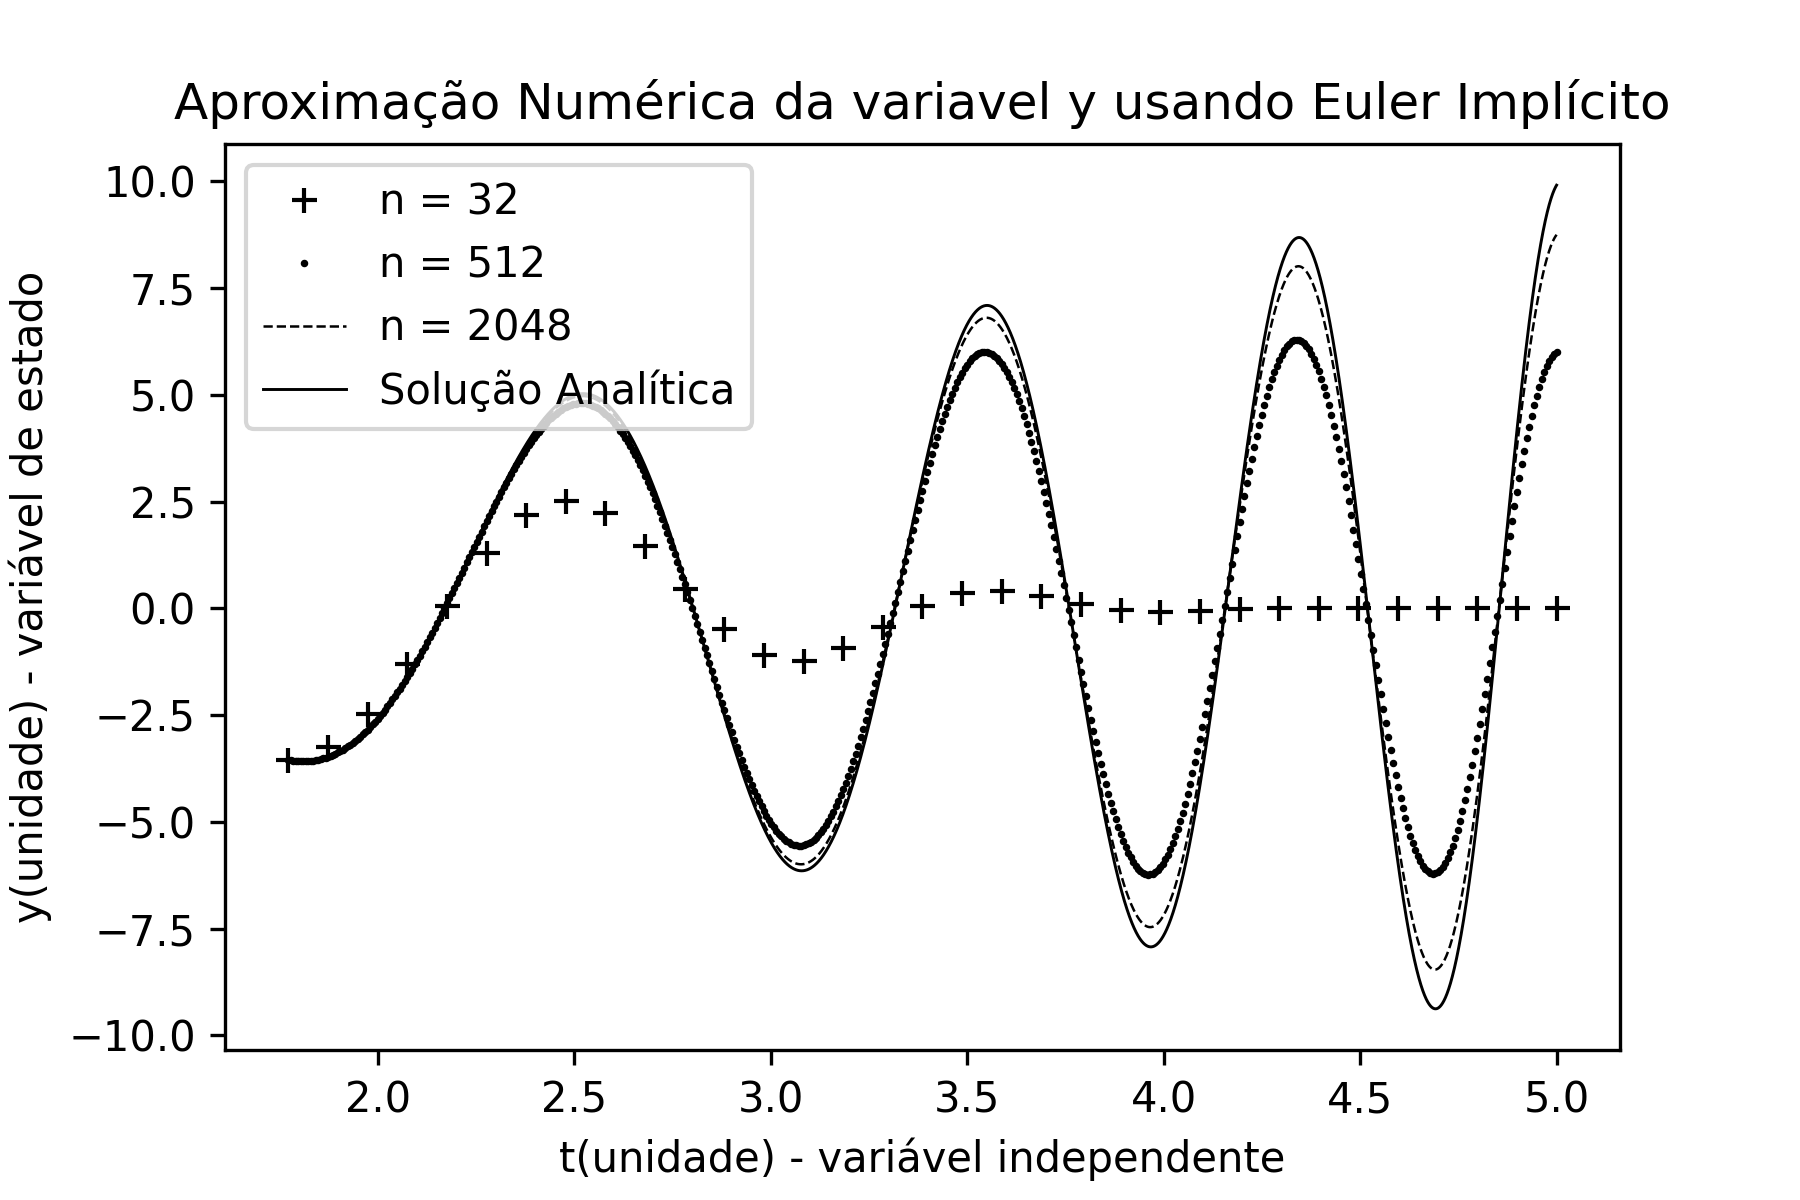
\includegraphics[scale=0.55]{images/metodo_2y_T5.0.png}
\caption{Aproximações numéricas da variável $y$ no intervalo $[\sqrt{\pi},5]$ para o Método de Euler Implícito.}
\label{fig:m2t5}
\end{figure}

%   TABELA EULER IMP T=3
\begin{table}[H]
 \centering
 \begin{tabular}{ c|c|c|c }
  \hline
  \hline
  $n$  & $\|e(t,h)\|$  & $q=\frac{\|e(t,2h)\|}{\|e(t,h)\|}$ & $\log_2(q)$ \\
  \hline
  \hline
$32$&$2.303830288$&	$$ &	$$ \\
\hline
$64$&$1.274448459$&$	1.807707697$&$	0.854161415$\\
\hline
$128$&$0.666786808$&$	1.911328245$&$	0.934575563
$\\
\hline
$256$&$0.340400628$&$	1.958829548$&$	0.969991864
$\\
\hline
$512$&$0.171885276$&$	1.980394342$&$	0.985787733
$\\
\hline
$1024$&$0.086354238$&$	1.99046718$&$	0.993107083
$\\
\hline
$2048$&$0.04327873$&$	1.995304326$&$	0.996608805
$\\
\hline
$4096$&$0.021664602$&$	1.997670257$&$	0.998318466
$\\
\hline
$8192$&$0.010838589$&$	1.998839704$&$	0.99916278
$\\
\hline
$16384$&$0.005420864$&$	1.999421002$&$	0.999582281
$\\
\hline
$32768$&$0.002710824$&$	1.999710789$&$	0.999791364
$\\
  \hline
  \hline
 \end{tabular}
   \caption{Estimação da ordem de convergência do Método de Euler Implícito no instante $T=3$, para o PVI com solução conhecida.} \label{tab:m2t3}
\end{table}


%   TABELA EULER IMP T=5
\begin{table}[H]
 \centering
 \begin{tabular}{ c|c|c|c }
  \hline
  \hline
  $n$  & $\|e(t,h)\|$  & $q=\frac{\|e(t,2h)\|}{\|e(t,h)\|}$ & $\log_2(q)$ \\
  \hline
  \hline
$32$&$9.912027698$&	$$ &	$$ \\
\hline
$64$&$9.765861212$&$	1.014967086$&$	0.021432944$\\
\hline
$128$&$8.592104495$&$	1.136608757$&	$0.184735736$\\
\hline
$256$&$6.28347663$&$	1.367412501$&$	0.45144852
$\\
\hline
$512$&$3.90395348$&$	1.609516267$&$	0.686627158$\\
\hline
$1024$&$2.189137223$&$	1.783329724$&$	0.834573471$\\
\hline
$2048$&$1.160669414$&$	1.886098829$&$	0.915405273$\\
\hline
$4096$&$0.597774563	$&$1.941650725	$&$0.957283704$\\
\hline
$8192$&$0.303365505	$&$1.970476387	$&$0.978544461$\\
\hline
$16384$&$0.152817333	$&$1.985151151	$&$0.989248859$\\
\hline
$32768$&$0.076694205	$&$1.992553848	$&$0.994618713$\\
  \hline
  \hline
 \end{tabular}
   \caption{Estimação da ordem de convergência do Método de Euler Implícito no instante $T=5$, para o PVI com solução conhecida.} \label{tab:m2t5}
\end{table}


\subsubsection{Resultados do Método do Trapézio Implícito}
O método do trapézio implícito mostrou a maior eficiência na reconstrução da solução. As Figuras \ref{fig:m3t3} e \ref{fig:m3t5} apresentam os diagramas comparando as soluções exatas e aproximadas para $n=32,512,2048$.

No que lhe concerne, as Tabelas \ref{tab:m3t3} e \ref{tab:m3t5} estimam a ordem de convergência deste método, que é aproximadamente $p=2$, o que explica a maior precisão mostrada nas soluções aproximadas.

\begin{figure}[H]
\centering
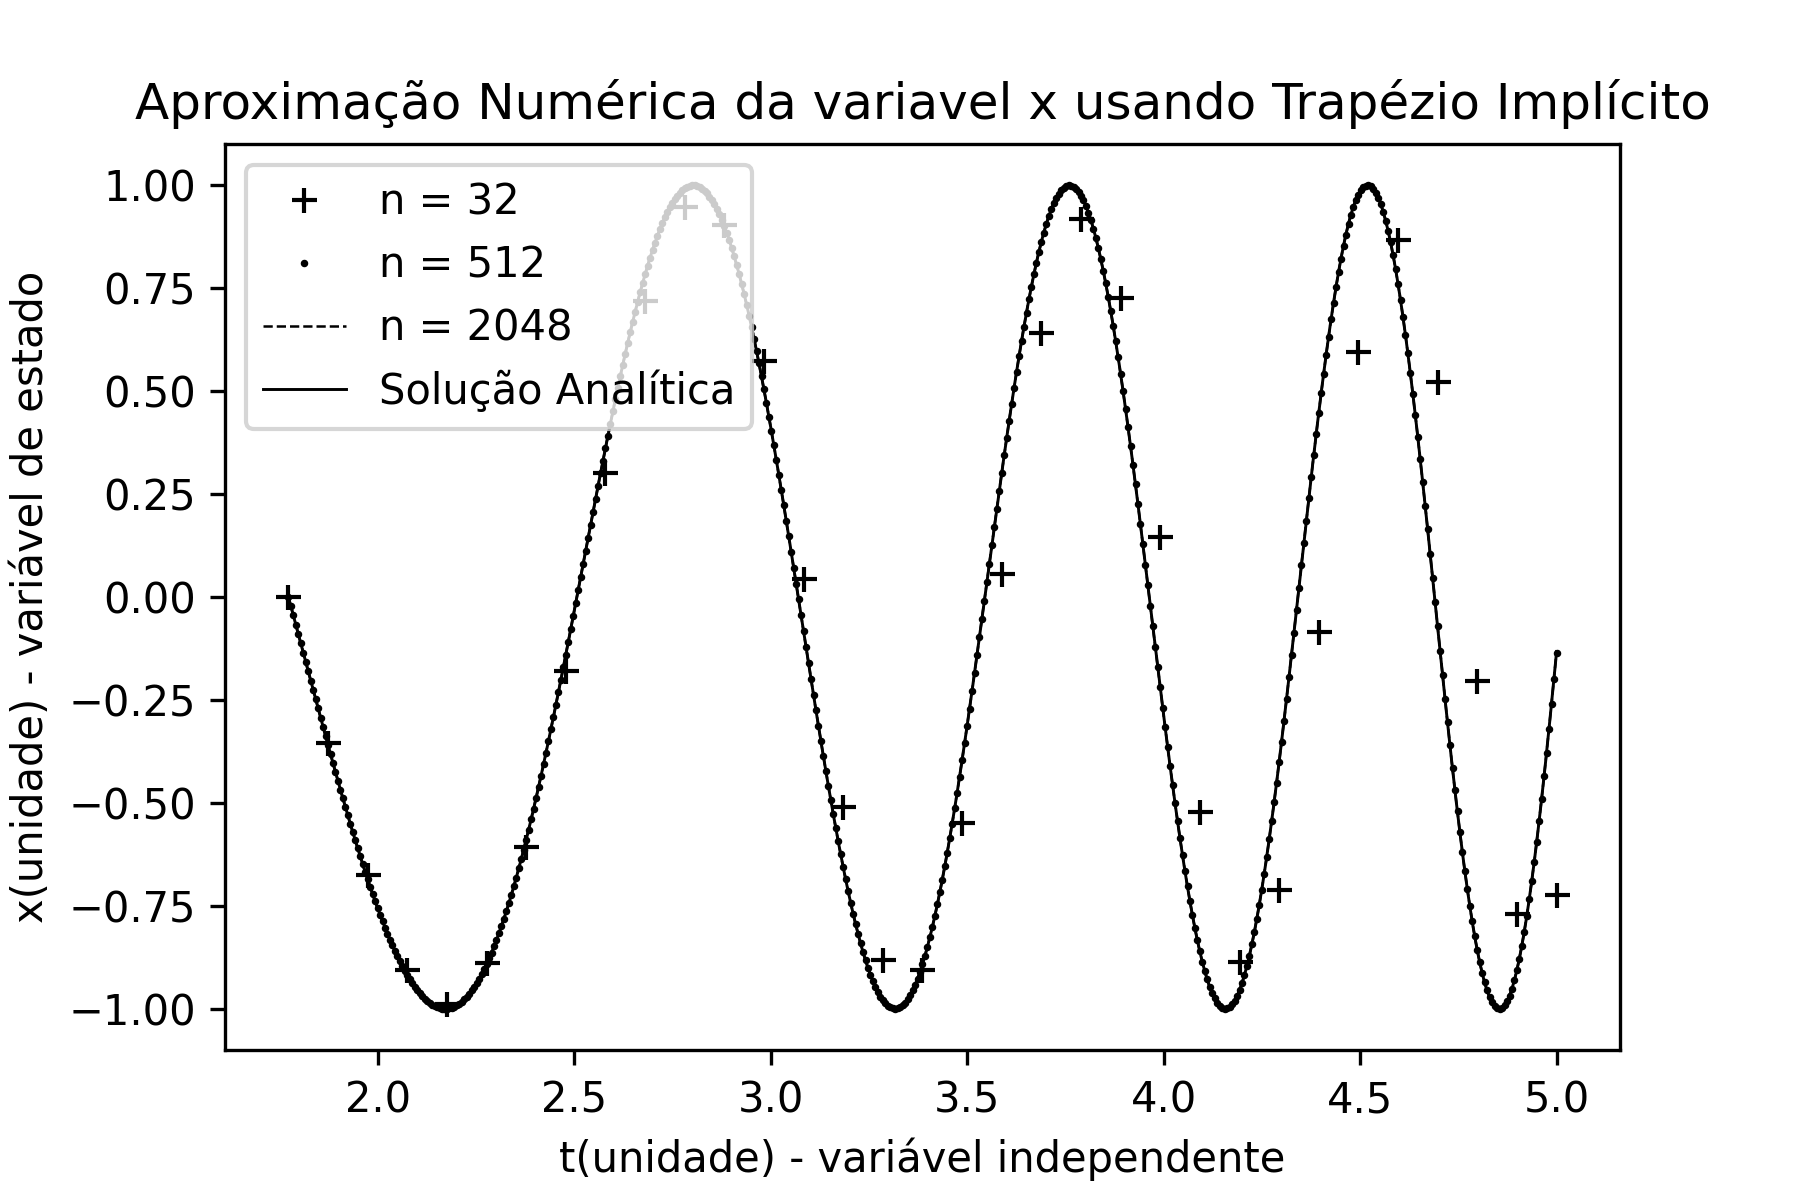
\includegraphics[scale=0.55]{images/metodo_3x_T5.0.png}
\caption{Aproximações numéricas da variável $x$ no intervalo $[\sqrt{\pi},5]$ para o Método do Trapézio Implícito.}
\label{fig:m3t3}
\end{figure}

\begin{figure}[H]
\centering
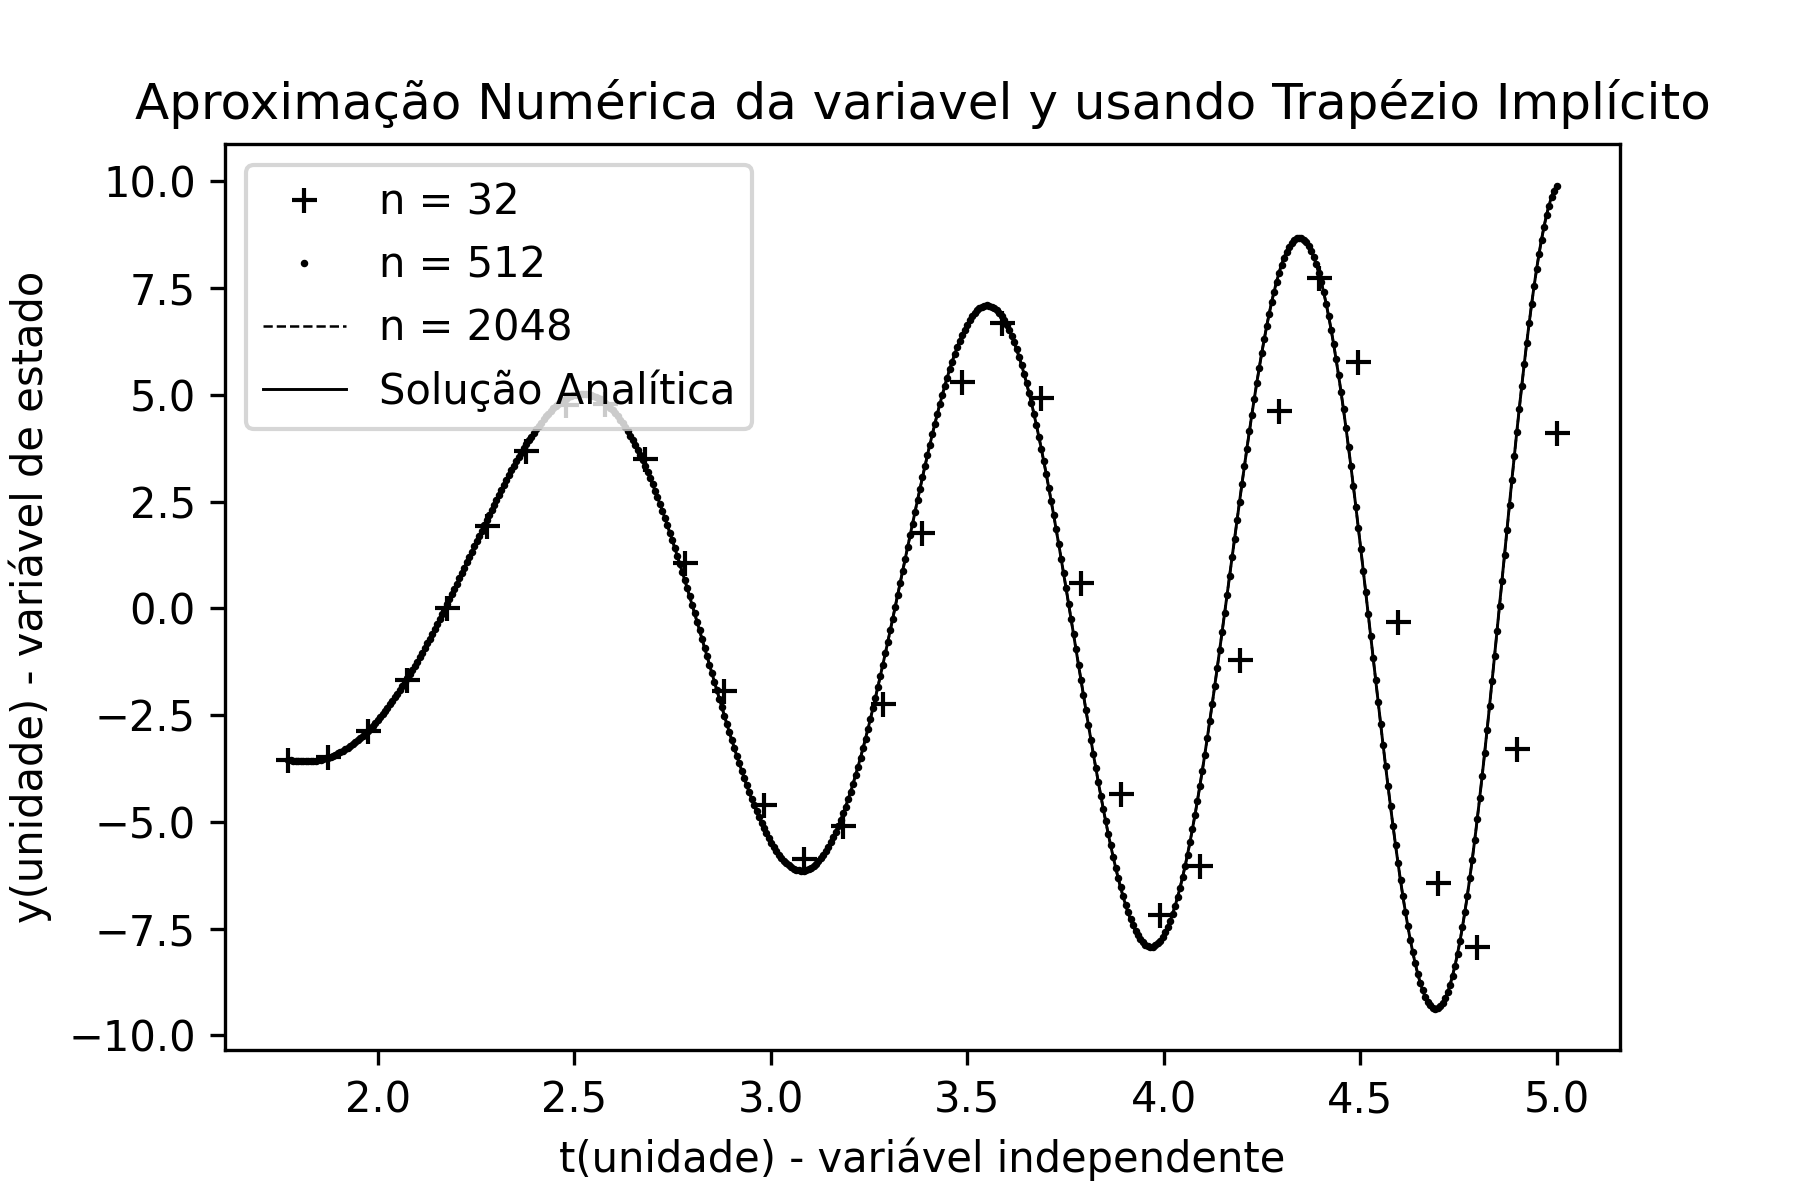
\includegraphics[scale=0.55]{images/metodo_3y_T5.0.png}
\caption{Aproximações numéricas da variável $y$ no intervalo $[\sqrt{\pi},5]$ para o Método de Euler Implícito.}
\label{fig:m3t5}
\end{figure}

%   TABELA TRAPEZIO T=3
\begin{table}[H]
 \centering
 \begin{tabular}{ c|c|c|c }
  \hline
  \hline
  $n$  & $\|e(t,h)\|$  & $q=\frac{\|e(t,2h)\|}{\|e(t,h)\|}$ & $\log_2(q)$ \\
  \hline
  \hline
$32$&$0.077050622$&	$$ &	$$ \\
\hline
$64$&$0.019291708	$&$3.993976112	$&$1.997825704$\\
\hline
$128$&$0.004824726	$&$3.998508761	$&$1.999462049$\\
\hline
$256$&$0.001206293	$&$3.999628791	$&$1.999866108$\\
\hline
$512$&$0.00030158	$&$3.999907321	$&$1.999966573$\\
\hline
$1024$&$0.000075396	$&$3.999976839	$&$1.999991646$\\
\hline
$2048$&$0.000018849	$&$3.999994209	$&$1.999997911$\\
\hline
$4096$&$0.000004712	$&$3.999998538	$&$1.999999473$\\
\hline
$8192$&$0.000001178	$&$3.999999607	$&$1.999999858$\\
\hline
$16384$&$0.000000295	$&$4.000000238	$&$2.000000086$\\
\hline
$32768$&$0.000000074	$&$4.000001122	$&$2.000000405$\\
  \hline
  \hline
 \end{tabular}
   \caption{Estimação da ordem de convergência do Método do Trapézio Implícito no instante $T=3$, para o PVI com solução conhecida.} \label{tab:m3t3}
\end{table}


%   TABELA TRAPEZIO T=5
\begin{table}[H]
 \centering
 \begin{tabular}{ c|c|c|c }
  \hline
  \hline
  $n$  & $\|e(t,h)\|$  & $q=\frac{\|e(t,2h)\|}{\|e(t,h)\|}$ & $\log_2(q)$ \\
  \hline
  \hline
$32$&$5.799582249$&	$$ &	$$ \\
\hline
$64$&$1.015490991	$&$5.711111473	$&$2.513771544$\\
\hline
$128$&$0.206736202	$&$4.912013372	$&$2.296314488$\\
\hline
$256$&$0.048430371	$&$4.268730535	$&$2.093807095$\\
\hline
$512$&$0.011899117	$&$4.070080973	$&$2.025057497$\\
\hline
$1024$&$0.002961667	$&$4.017709857	$&$2.006373382$\\
\hline
$2048$&$0.000739596	$&$4.004439513	$&$2.001600328$\\
\hline
$4096$&$0.000184848	$&$4.001110636	$&$2.000400522$\\
\hline
$8192$&$0.000046209	$&$4.000277707	$&$2.000100158$\\
\hline
$16384$&$0.000011552	$&$4.000069431	$&$2.000025042$\\
\hline
$32768$&$0.000002888	$&$4.000017488	$&$2.000006307$\\
  \hline
  \hline
 \end{tabular}
   \caption{Estimação da ordem de convergência do Método do Trapézio Implícito no instante $T=5$, para o PVI com solução conhecida.} \label{tab:m3t5}
\end{table}
%=============================================================
%   CASO 2
\subsection{Problema de Cauchy genérico}
Nesta seção de exemplos, serão realizadas aproximações numéricas da ordem de convergência dos métodos: Euler, Euler implícito e Trapézio, no problema de Cauchy \eqref{eq:EDO}, sem considerar a solução analítica como mostrado na seção $2.3.3$ em \cite{livroProfAlexandre}. Ou seja, dado $T$ fixo e $h2^m=(T-\sqrt{\pi})$, $m=5,6,7,...,15$ o tamanho de passo de integração do método usado.
Se $\tilde{y}(t,h2^i),\, \tilde{y}(t,h2^{i-1}),\, \tilde{y}(t,h/2^{i-2})$ são as soluções numéricas correspondentes aos passos de integração em $h2^i,\, h2^{i-1}$ e $h2^{i-2}$ para $i=7,8,9,...,15$ correspondentemente.
Então, uma estimativa para a ordem de convergência do método usado, é dada por:
\begin{equation}
    \tilde{p}=\log_2\left(\frac{\|\tilde{y}(t,h2^i)-\tilde{y}(t,h2^{i-1})\|}{\|\tilde{y}(t,h2^{i-1})-\tilde{y}(t,h2^{i-2})\|} \right).
\end{equation}
Onde, $\| . \|$, denota a norma do máximo.

A seguir, os resultados obtidos para cada um dos métodos mencionado são mostrados.

\subsubsection{Resultados para o Método de Euler}
A Tabela \ref{tab:c2m1t3}, mostra estimativas da ordem de convergência do Método de Euler, para o instante fixo $T=3$, considerando uma partição de $n=2^m$ subintervalos do intervalo $[\sqrt{\pi}, T]$. Os resultados sugerem que a ordem de convergência do Método de Euler tende para $1$, sendo esta, a ordem de convergência prevista pela teoria à medida que o passo de integração se aproxima de zero.

%   TABELA MET 1 T 3
\begin{table}[H]
 \centering
 \begin{tabular}{ c|c|c|c }
  \hline
  \hline
  $n$  & $h$  & $\tilde{y}(t,h)$ & $\tilde{p}$ \\
  \hline
  \hline
$32$&$0.03836$&	$ (0.93586, -8.45743)$ &	$ $ \\
\hline
$64$&$0.01918$&$ (0.61651,-6.93800)$&$ $\\
\hline
$128$&$0.00959	 $&$(   0.50189,   -6.18437)$&$	1.01E+00$\\
\hline
$256$&$0.0048	 $&$(   0.45416,   -5.81998)	$&$1.05E+00$\\
\hline
$512$&$0.0024	 $&$(   0.43246,   -5.64187)	$&$1.03E+00$\\
\hline
$1024$&$0.0012	 $&$(   0.42212,   -5.55394)	$&$1.02E+00$\\
\hline
$2048$&$0.0006	 $&$(   0.41708,   -5.51026)	$&$1.01E+00$\\
\hline
$4096$&$0.0003	 $&$(   0.41459,   -5.48850)	$&$1.00E+00$\\
\hline
$8192$&$0.00015	 $&$(   0.41335,   -5.47763)	$&$1.00E+00$\\
\hline
$16384$&$0.00007	 $&$(   0.41273,   -5.47221)	$&$1.00E+00$\\
\hline
$32768$&$0.00004	 $&$(   0.41243,   -5.46949)	$&$1.00E+00$\\
  \hline
  \hline
 \end{tabular}
   \caption{Estimação da ordem de convergência do Método de Euler no instante $T=3$, para o PVI genérico.} \label{tab:c2m1t3}
\end{table}

Por outro lado, a Tabela \ref{tab:c2m1t5}, considera o instante de tempo $T=5$, e estima também, uma ordem de convergência de $1$. Onde, além disso, podemos perceber que para $n=256$, obtemos um valor negativo para a estimativa numérica de $\tilde{p}=-1.34\times 10^{-3}$, o que não é preocupante, uma vez que $\tilde{p}$ tende ao valor esperado $1$ à medida que $h$ se aproxima de zero.

Estas estimativas são as mesmas que as obtidas no caso en que se considerou a solução exata para calcular a ordem de convergência $p$ usando a solução exata (seção \ref{sec:PVIConSol}).

%   TABELA MET 1 T 5
\begin{table}[H]
 \centering
 \begin{tabular}{ c|c|c|c }
  \hline
  \hline
  $n$  & $h$  & $\tilde{y}(t,h)$ & $\tilde{p}$ \\
  \hline
  \hline
$32$&$0.10086$&	$  ( 183.56335, -3585.57970)$ &	$ $ \\
\hline
$64$&$0.05043$&$  ( -37.44513,   76.20665)$&$ $\\
\hline
$128$&$0.02522	 $&$  (  -3.62784,   59.80913)	$&$6.76E+00$\\
\hline
$256$&$0.01261	 $&$  (  -0.74186,   25.96045)	$&$-1.34E-03$\\
\hline
$512$&$0.0063	 $&$  (  -0.31085,   16.19399)	$&$1.79E+00$\\
\hline
$1024$&$0.00315	 $&$  (  -0.20111,   12.69133)	$&$1.48E+00$\\
\hline
$2048$&$0.00158	 $&$  (  -0.16262,   11.21996)	$&$1.25E+00$\\
\hline
$4096$&$0.00079	 $&$  (  -0.14657,   10.54660)	$&$1.13E+00$\\
\hline
$8192$&$0.00039	 $&$  (  -0.13924,   10.22459)	$&$1.06E+00$\\
\hline
$16384$&$0.0002	 $&$  (  -0.13574,   10.06715)	$&$1.03E+00$\\
\hline
$32768$&$0.0001	 $&$  (  -0.13403,    9.98930)	$&$1.02E+00$\\
  \hline
  \hline
 \end{tabular}
   \caption{Estimação da ordem de convergência do Método de Euler no instante $T=5$, para o PVI genérico.} \label{tab:c2m1t5}
\end{table}

\subsubsection{Resultados para o Método de Euler Implícito}
Considerando o instante fixo $T=3$. Utilizando as soluções numéricas, obtemos uma estimativa da ordem de convergência do método de Euler Implícito, obtemos $\tilde{p}=1$, ver Tabela \ref{tab:c2m2t3}, como esperado, sendo este valor o mesmo, comparado com o resultado encontrado na Tabela \ref{tab:m2t3} do exemplo análogo.
%   TABELA MET 2 T 3
\begin{table}[H]
 \centering
 \begin{tabular}{ c|c|c|c }
  \hline
  \hline
  $n$  & $h$  & $\tilde{y}(t,h)$ & $\tilde{p}$ \\
  \hline
  \hline
$32$&$0.03836$&	$  (   0.22252,   -3.16295)$ &	$ $ \\
\hline
$64$&$0.01918$&$  (   0.29075,   -4.19233)$&$ $\\
\hline
$128$&$0.00959	 $&$  (   0.34306,   -4.79999)	$&$7.60E-01$\\
\hline
$256$&$0.0048	 $&$ (   0.37526,   -5.12638)	$&$8.97E-01$\\
\hline
$512$&$0.0024	 $&$  (   0.39307,   -5.29490)	$&$9.54E-01$\\
\hline
$1024$&$0.0012	 $&$  (   0.40244,   -5.38043)	$&$9.78E-01$\\
\hline
$2048$&$0.0006	 $&$  (   0.40724,   -5.42350)	$&$9.90E-01$\\
\hline
$4096$&$0.0003	 $&$  (   0.40967,   -5.44512)	$&$9.95E-01$\\
\hline
$8192$&$0.00015	 $&$  (   0.41089,   -5.45594)	$&$9.97E-01$\\
\hline
$16384$&$0.00007	 $&$  (   0.41150,   -5.46136)	$&$9.99E-01$\\
\hline
$32768$&$0.00004	 $&$ (   0.41181,   -5.46407)	$&$9.99E-01$\\
  \hline
  \hline
 \end{tabular}
   \caption{Estimação da ordem de convergência do Método de Euler Implícito no instante $T=3$, para o PVI genérico.} \label{tab:c2m2t3}
\end{table}

Entretanto, a Tabela \ref{tab:c2m2t5}, também mostra um resultado esperado, $\tilde{p}=1$, da ordem de convergência do método de Euler Implícito, conforme $h$ tende a zero, para $ T=5$; comparado com o exemplo análogo, veja a Tabela \ref{tab:m2t5}.

%   TABELA MET 2 T 5
\begin{table}[H]
 \centering
 \begin{tabular}{ c|c|c|c }
  \hline
  \hline
  $n$  & $h$  & $\tilde{y}(t,h)$ & $\tilde{p}$ \\
  \hline
  \hline
$32$&$0.10086$&	$    (   0.00000,    0.00000)$ &	$ $ \\
\hline
$64$&$0.05043$&$   (  -0.01449,    0.14617)$&$ $\\
\hline
$128$&$0.02522	 $&$    (  -0.03067,    1.31992)	$&$-3.01E+00$\\
\hline
$256$&$0.01261	 $&$  (  -0.04251,    3.62855)	$&$-9.76E-01$\\
\hline
$512$&$0.0063	 $&$    (  -0.06536,    6.00807)$&$-4.36E-02$\\
\hline
$1024$&$0.00315	 $&$    (  -0.09035,    7.72289)	$&$4.73E-01$\\
\hline
$2048$&$0.00158	 $&$    (  -0.10871,    8.75136)	$&$7.38E-01$\\
\hline
$4096$&$0.00079	 $&$    (  -0.11979,    9.31425)	$&$8.70E-01$\\
\hline
$8192$&$0.00039	 $&$    (  -0.12588,    9.60866)	$&$9.35E-01$\\
\hline
$16384$&$0.0002	 $&$    (  -0.12906,    9.75921)	$&$9.68E-01$\\
\hline
$32768$&$0.0001	 $&$   (  -0.13069,    9.83533)	$&$9.84E-01$\\
  \hline
  \hline
 \end{tabular}
   \caption{Estimação da ordem de convergência do Método de Euler Implícito no instante $T=5$, para o PVI genérico.} \label{tab:c2m2t5}
\end{table}

\subsubsection{Resultados para o Método do Trapézio Implícito}
Como último caso, mostramos nas Tabelas \ref{tab:c2m3t3} e \ref{tab:c2m1t5}, uma estimativa da ordem de convergência do método do Trapézio para os instantes $T=3$ e $T=5$, sendo esta ordem $\tilde{p}=2$, quando $h$ tende a zero; o que se enquadra nos resultados obtidos nos respectivos casos análogos da seção anterior \ref{sec:PVIConSol}, ver Tabelas \ref{tab:m3t3} e \ref{tab:m3t5}.
%   TABELA MET 3 T 3
\begin{table}[H]
 \centering
 \begin{tabular}{ c|c|c|c }
  \hline
  \hline
  $n$  & $h$  & $\tilde{y}(t,h)$ & $\tilde{p}$ \\
  \hline
  \hline
$32$&$0.03836$&	$   (   0.42495,   -5.38973)$ &	$ $ \\
\hline
$64$&$0.01918$&$   (   0.41537,   -5.44749)$&$ $\\
\hline
$128$&$0.00959	 $&$   (   0.41293,   -5.46196)	$&$2.00E+00$\\
\hline
$256$&$0.0048	 $&$  (   0.41232,   -5.46558)	$&$2.00E+00$\\
\hline
$512$&$0.0024	 $&$   (   0.41217,   -5.46648)	$&$2.00E+00$\\
\hline
$1024$&$0.0012	 $&$   (   0.41213,   -5.46671)	$&$2.00E+00$\\
\hline
$2048$&$0.0006	 $&$   (   0.41212,   -5.46676)	$&$2.00E+00$\\
\hline
$4096$&$0.0003	 $&$   (   0.41212,   -5.46678)	$&$2.00E+00$\\
\hline
$8192$&$0.00015	 $&$   (   0.41212,   -5.46678)	$&$2.00E+00$\\
\hline
$16384$&$0.00007	 $&$   (   0.41212,   -5.46678)	$&$2.00E+00$\\
\hline
$32768$&$0.00004	 $&$  (   0.41212,   -5.46678)	$&$2.00E+00$\\
  \hline
  \hline
 \end{tabular}
   \caption{Estimação da ordem de convergência do Método do Trapézio Implícito no instante $T=3$, para o PVI genérico.} \label{tab:c2m3t3}
\end{table}
%   TABELA MET 3 T 5
\begin{table}[H]
 \centering
 \begin{tabular}{ c|c|c|c }
  \hline
  \hline
  $n$  & $h$  & $\tilde{y}(t,h)$ & $\tilde{p}$ \\
  \hline
  \hline
$32$&$0.10086$&	$    (  -0.72337,    4.11245)$ &	$ $ \\
\hline
$64$&$0.05043$&$    (  -0.36173,    8.89654)$&$ $\\
\hline
$128$&$0.02522	 $&$    (  -0.19405,    9.70529)	$&$2.56E+00$\\
\hline
$256$&$0.01261	 $&$   (  -0.14803,    9.86360)	$&$2.35E+00$\\
\hline
$512$&$0.0063	 $&$    (  -0.13629,    9.90013)	$&$2.12E+00$\\
\hline
$1024$&$0.00315	 $&$    (  -0.13334,    9.90907)	$&$2.03E+00$\\
\hline
$2048$&$0.00158	 $&$    (  -0.13260,    9.91129)	$&$2.01E+00$\\
\hline
$4096$&$0.00079	 $&$    (  -0.13241,    9.91184)	$&$2.00E+00$\\
\hline
$8192$&$0.00039	 $&$    (  -0.13237,    9.91198)	$&$2.00E+00$\\
\hline
$16384$&$0.0002	 $&$    (  -0.13236,    9.91202)	$&$2.00E+00$\\
\hline
$32768$&$0.0001	 $&$   (  -0.13235,    9.91203)	$&$2.00E+00$\\
  \hline
  \hline
 \end{tabular}
   \caption{Estimação da ordem de convergência do Método do Trapézio Implícito no instante $T=5$, para o PVI genérico.} \label{tab:c2m3t5}
\end{table}

\section{Conclusões}
O objetivo deste trabalho foi estudar a convergência de três métodos numéricos (Euler, Euler Implícito e Trapézio Implícito), aplicados a um determinado problema com solução analítica.

Mediante exemplos numéricos, estes métodos foram comparados para um intervalo contendo a solução e também os erros para os instantes $T=3$ e $T=5$. Primeiro, as ordens de convergência foram estimadas considerando a solução exata e depois, outro procedimento foi realizado sem considerar a solução analítica. Em todos os casos, comportamentos similares foram obtidos à medida que o tamanho do passo de integração se aproximava de zero.

\newpage

\bibliographystyle{plain}
\bibliography{biblio}


\end{document}
